\newpage
\section{Parallelism}
\subsection{Instruction Parallelism}

\subsubsection{Co-Processors}

\begin{figure}[h!]
\centering
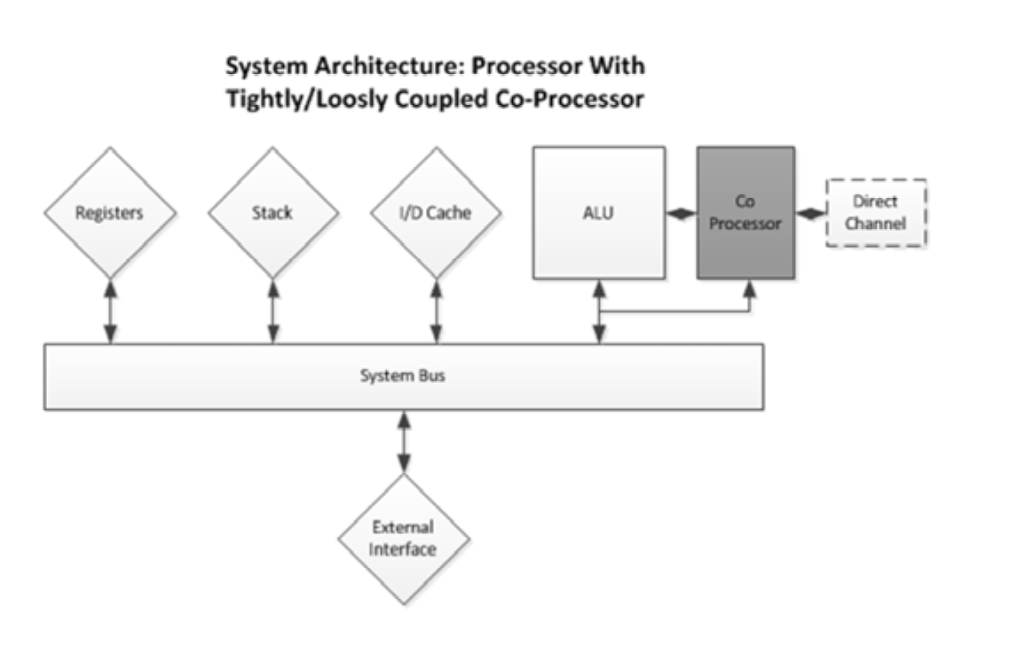
\includegraphics[width=13cm]{pic/co_processor}
\caption{Co-Processor}
\end{figure}
A classical Co-Processor is a device that has its own instruction set. The use of this device is triggered by co-processor instructions in the program code.\newline


1.) The processor receives an Unidentified instruction \newline
2.) The processor will (generally) ask its co-processors whether this instruction applies to them\newline
3.) If no then it generates a unidentified op-code exception and lets normal exception processing take over\newline
4.) Co-Processors will listen to the instruction and identify themselves\newline
5.) The instruction is passed for processing to the co-processor.\newline
6.) A processor will continue to execute instructions whilst the co-processor is doing its bit.\newline
7.) If the co-processor is busy and the processor has a co-processor instruction next in its stream – the processor will stall\newline
8.) A co-processor will generally have some form of exception registration\newline


\subsection{Instruction Parallelism}
\begin{figure}[H]
\centering
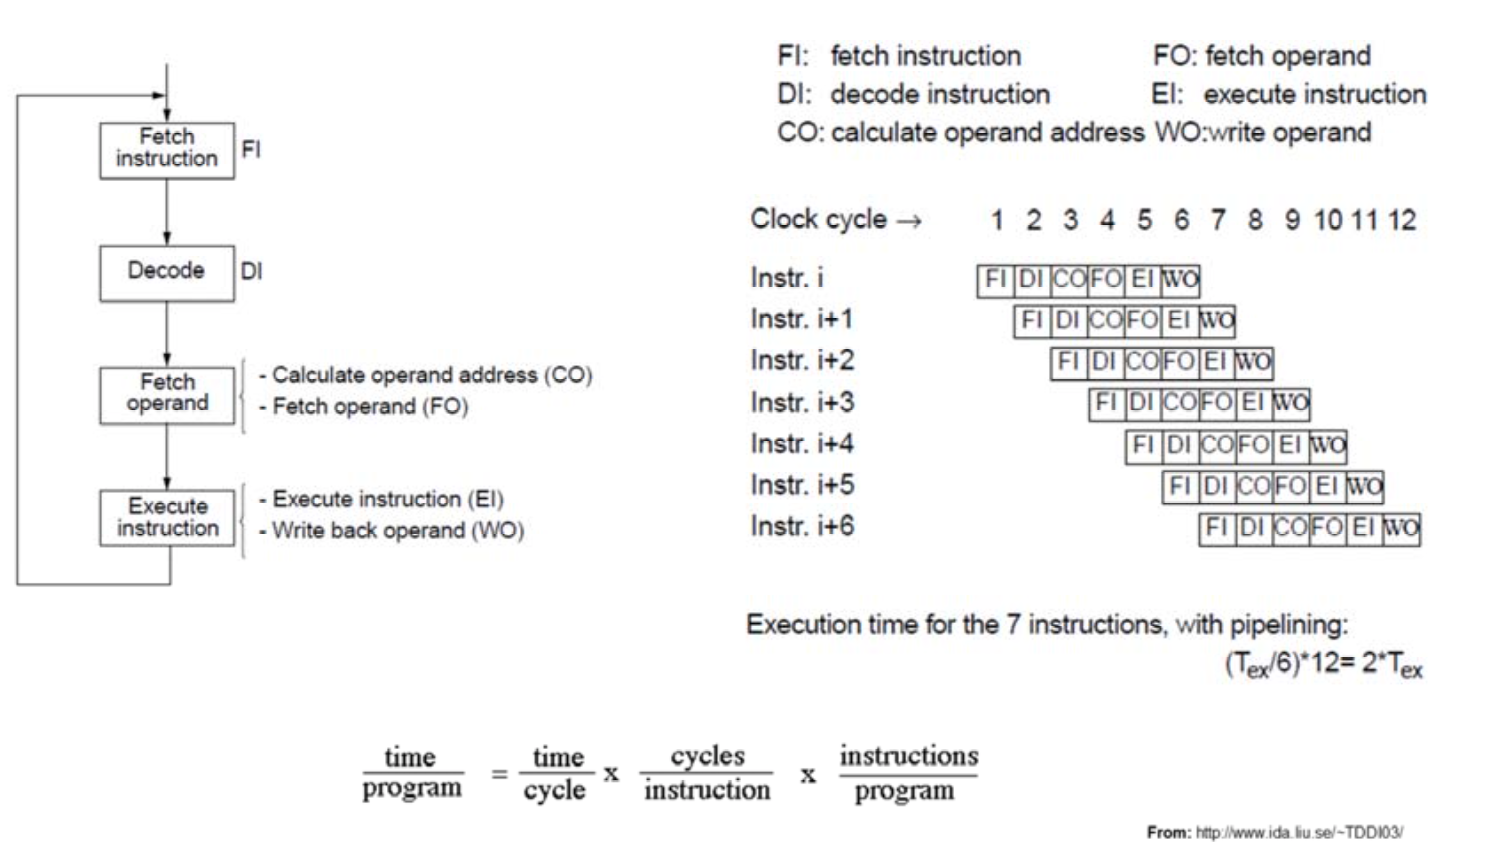
\includegraphics[width=13cm]{pic/instruction_parallelism}
\caption{Instruction Parallelism}
\end{figure}

\subsubsection{Hazards}

Structural hazards occur when a certain resource (memory, functional unit) is requested by more than one instruction at the same time. For instance if a memory is unable to accept another transfer with a clock cycle then the pipeline is stalled for a clock cycle. Certain resources can be duplicated in order to avoid structural hazards. Functional units (ALU, FP unit) can be pipelined themselves in order to support several instructions at a time. A classical way to avoid hazards at memory access is by providing separate data and instruction caches. \newline

\begin{figure}[H]
\centering
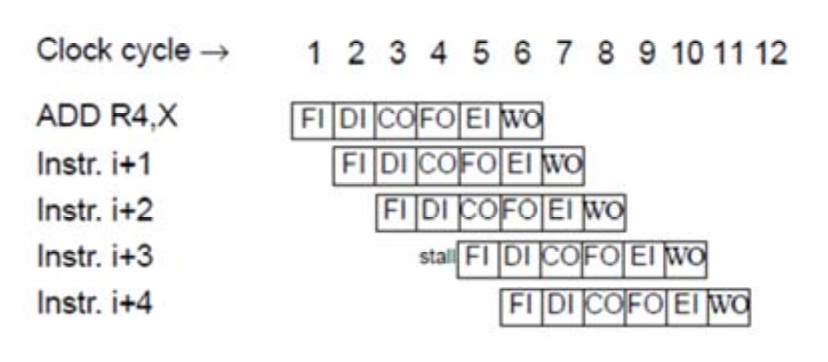
\includegraphics{pic/structural_hazard}
\caption{Structural Hazzard}
\end{figure}


Data Hazards We have two instructions, I1 and I2. In a pipeline the execution of I2 can start before I1 has terminated. If in a certain stage of the pipeline, I2 needs the result produced by I1, but this result has not yet been generated, we have a data hazard. Some of the penalty produced by data hazards can be avoided using a technique called forwarding (bypassing). \newline

\begin{figure}[H]
\centering
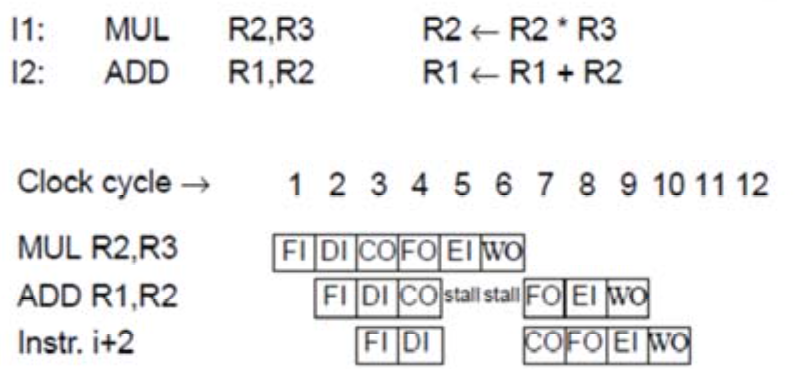
\includegraphics{pic/data_hazard}
\caption{Data Hazzard}
\end{figure}


Control hazards are produced by branch instructions. Branch instructions represent a major problem in assuring an optimal flow through the pipeline. Several approaches have been taken for reducing branch penalties. \newline
\begin{figure}[H]
\centering
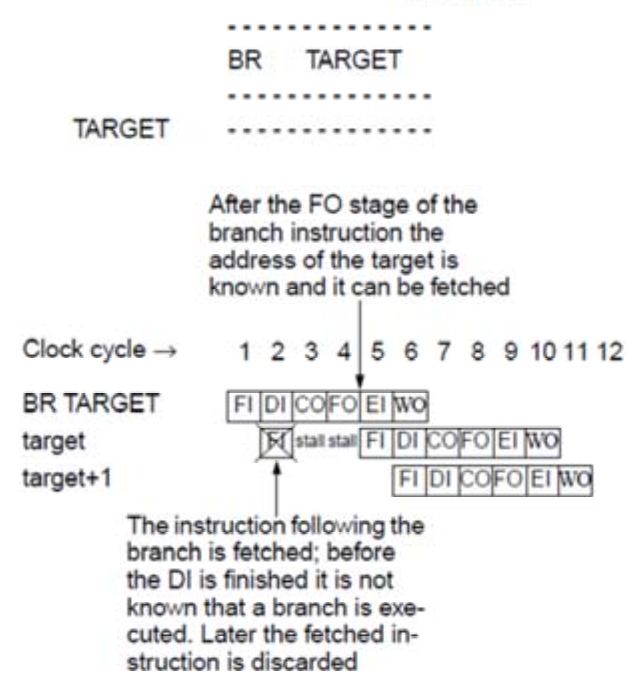
\includegraphics{pic/ctrl_hazard}
\caption{Data Hazzard}
\end{figure}


